%\documentclass[%
%% border=1pt
%  border={0pt 0pt 0pt 0pt} % left bottom right top
%]{standalone}
%\usepackage{tikz} % Required for drawing custom shapes
%\usepackage{pgfplots}
%\pgfplotsset{compat = newest}
%
%\usepackage{amsbsy}
%\usetikzlibrary{decorations.pathreplacing,calc}
%\usetikzlibrary{shapes}
%\usepackage{amsmath,stackrel}
%\usetikzlibrary{arrows.meta}
%\usetikzlibrary{arrows}
%\usetikzlibrary{calc}
%\usetikzlibrary{math}
%
%\begin{document}
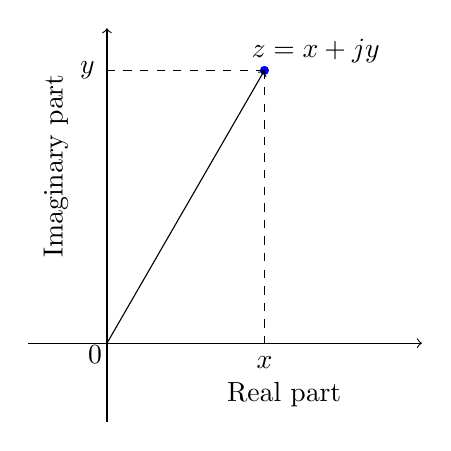
\begin{tikzpicture}
\draw[black,->] (-1,0) -- (4,0);
\draw[black,->] (0,-1) -- (0,4);
\draw[fill,blue] (2,{2*sqrt(3)}) circle[radius=0.05];
\node[align=left,rotate=90] at (-0.65,2.25){Imaginary part};
\node[align=left,rotate=0] at (2.25,-0.65){Real part};
\node at (-0.15,-0.15){0};
\draw[black,->] (0,0) -- (2,{2*sqrt(3)});
\node at (2.65,{2*sqrt(3)+0.25}) {$z = x + j y$};
\draw[dashed] (2,{2*sqrt(3)}) -- (0,{2*sqrt(3)});
\draw[dashed] (2,{2*sqrt(3)}) -- (2,0);
\node at (2,-0.25){$x$};
\node at (-0.25,{2*sqrt(3)}){$y$};
\end{tikzpicture}
%\end{document}